\documentclass{standalone}
\usepackage{tikz}
\usetikzlibrary{patterns, positioning}

\begin{document}
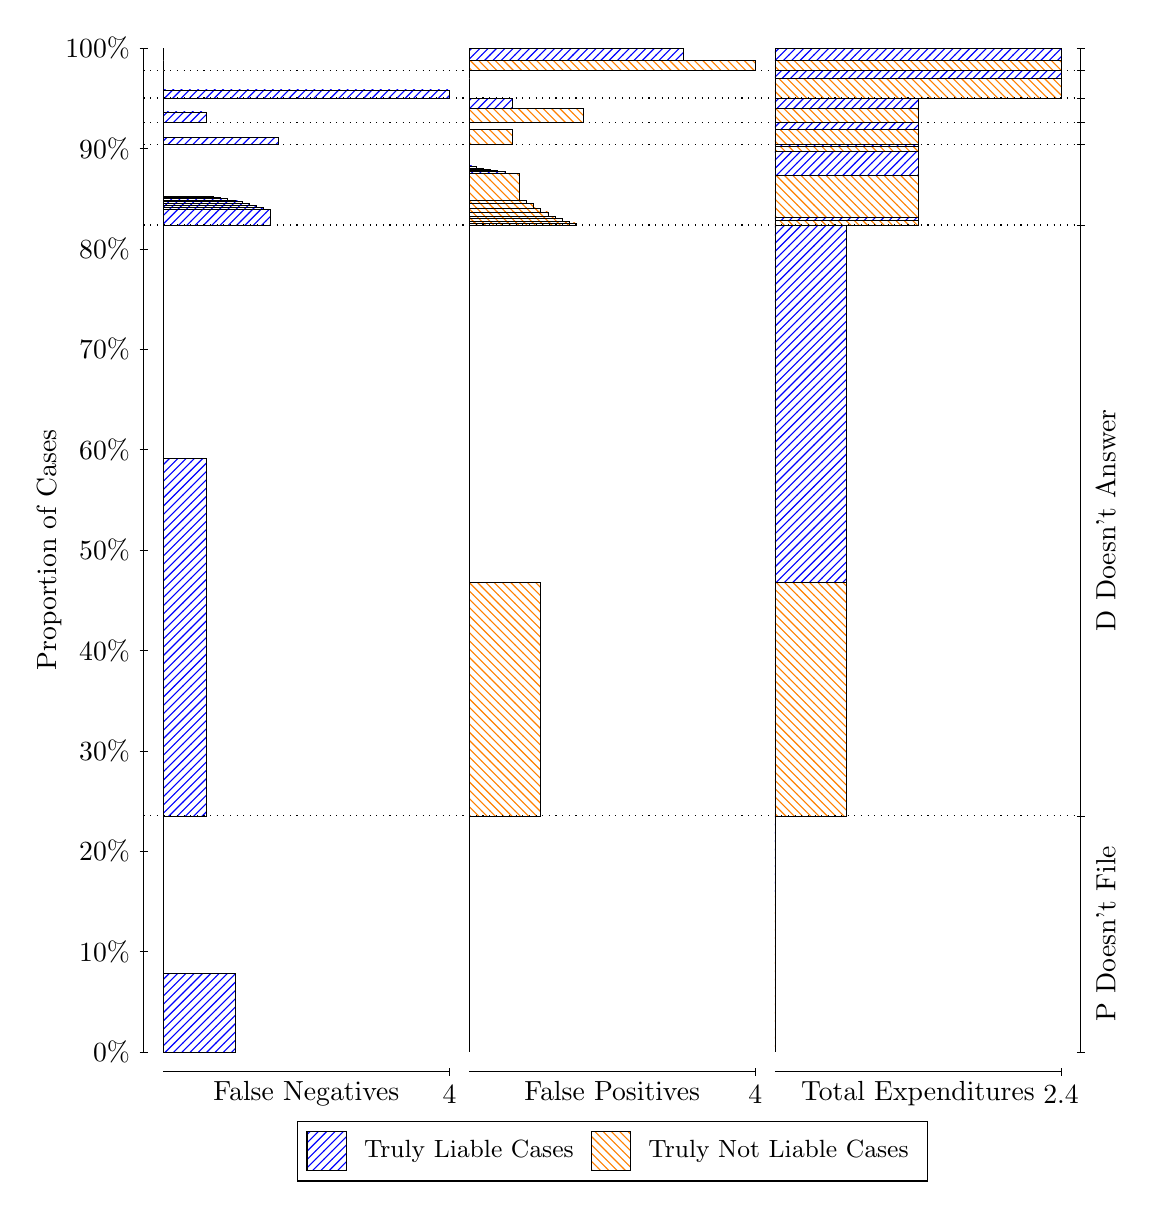
\begin{tikzpicture}
\draw[black, very thin] (1.5,1.75) -- (1.5,14.5);
\node[rotate=90, anchor=center] at (0.3, 8.125) {Proportion of Cases};
\draw[black, very thin] (1.45,1.75) -- (1.55,1.75);
\node[anchor=east] at (1.45, 1.75) {0\%};
\draw[black, very thin] (1.45,3.025) -- (1.55,3.025);
\node[anchor=east] at (1.45, 3.025) {10\%};
\draw[black, very thin] (1.45,4.3) -- (1.55,4.3);
\node[anchor=east] at (1.45, 4.3) {20\%};
\draw[black, very thin] (1.45,5.575) -- (1.55,5.575);
\node[anchor=east] at (1.45, 5.575) {30\%};
\draw[black, very thin] (1.45,6.85) -- (1.55,6.85);
\node[anchor=east] at (1.45, 6.85) {40\%};
\draw[black, very thin] (1.45,8.125) -- (1.55,8.125);
\node[anchor=east] at (1.45, 8.125) {50\%};
\draw[black, very thin] (1.45,9.4) -- (1.55,9.4);
\node[anchor=east] at (1.45, 9.4) {60\%};
\draw[black, very thin] (1.45,10.675) -- (1.55,10.675);
\node[anchor=east] at (1.45, 10.675) {70\%};
\draw[black, very thin] (1.45,11.95) -- (1.55,11.95);
\node[anchor=east] at (1.45, 11.95) {80\%};
\draw[black, very thin] (1.45,13.225) -- (1.55,13.225);
\node[anchor=east] at (1.45, 13.225) {90\%};
\draw[black, very thin] (1.45,14.5) -- (1.55,14.5);
\node[anchor=east] at (1.45, 14.5) {100\%};

\draw[black, very thin] (13.4,1.75) -- (13.4,14.5);
\draw[black, very thin] (13.35,1.75) -- (13.45,1.75);
\node[anchor=west] at (13.35, 1.75) {};
\draw[black, very thin] (13.35,4.7496) -- (13.45,4.7496);
\node[anchor=west] at (13.35, 4.7496) {};
\draw[black, very thin] (13.35,12.252) -- (13.45,12.252);
\node[anchor=west] at (13.35, 12.252) {};
\draw[black, very thin] (13.35,13.277) -- (13.45,13.277);
\node[anchor=west] at (13.35, 13.277) {};
\draw[black, very thin] (13.35,13.553) -- (13.45,13.553);
\node[anchor=west] at (13.35, 13.553) {};
\draw[black, very thin] (13.35,13.865) -- (13.45,13.865);
\node[anchor=west] at (13.35, 13.865) {};
\draw[black, very thin] (13.35,14.212) -- (13.45,14.212);
\node[anchor=west] at (13.35, 14.212) {};
\draw[black, very thin] (13.35,14.5) -- (13.45,14.5);
\node[anchor=west] at (13.35, 14.5) {};

\draw[black, very thin, pattern color=blue, pattern=north east lines] (1.75,1.75) rectangle (2.6583,2.7436);
\draw[black, very thin, pattern color=orange, pattern=north west lines] (1.75,2.7436) rectangle (1.75,4.7496);
\draw[black, very thin, pattern color=blue, pattern=north east lines] (1.75,4.7496) rectangle (2.295,9.2841);
\draw[black, very thin, pattern color=orange, pattern=north west lines] (1.75,9.2841) rectangle (1.75,12.252);
\draw[black, very thin, pattern color=blue, pattern=north east lines] (1.75,12.252) rectangle (3.1125,12.45);
\draw[black, very thin, pattern color=blue, pattern=north east lines] (1.75,12.45) rectangle (3.0217,12.473);
\draw[black, very thin, pattern color=blue, pattern=north east lines] (1.75,12.473) rectangle (2.9308,12.5);
\draw[black, very thin, pattern color=blue, pattern=north east lines] (1.75,12.5) rectangle (2.84,12.527);
\draw[black, very thin, pattern color=blue, pattern=north east lines] (1.75,12.527) rectangle (2.7492,12.559);
\draw[black, very thin, pattern color=blue, pattern=north east lines] (1.75,12.559) rectangle (2.6583,12.568);
\draw[black, very thin, pattern color=blue, pattern=north east lines] (1.75,12.568) rectangle (2.5675,12.587);
\draw[black, very thin, pattern color=blue, pattern=north east lines] (1.75,12.587) rectangle (2.4767,12.599);
\draw[black, very thin, pattern color=blue, pattern=north east lines] (1.75,12.599) rectangle (2.3858,12.619);
\draw[black, very thin, pattern color=orange, pattern=north west lines] (1.75,12.619) rectangle (1.75,13.277);
\draw[black, very thin, pattern color=blue, pattern=north east lines] (1.75,13.277) rectangle (3.2033,13.363);
\draw[black, very thin, pattern color=orange, pattern=north west lines] (1.75,13.363) rectangle (1.75,13.553);
\draw[black, very thin, pattern color=blue, pattern=north east lines] (1.75,13.553) rectangle (2.295,13.688);
\draw[black, very thin, pattern color=orange, pattern=north west lines] (1.75,13.688) rectangle (1.75,13.865);
\draw[black, very thin, pattern color=blue, pattern=north east lines] (1.75,13.865) rectangle (5.3833,13.967);
\draw[black, very thin, pattern color=orange, pattern=north west lines] (1.75,13.967) rectangle (1.75,14.212);
\draw[black, very thin, pattern color=orange, pattern=north west lines] (1.75,14.212) rectangle (1.75,14.343);
\draw[black, very thin, pattern color=blue, pattern=north east lines] (1.75,14.343) rectangle (1.75,14.5);
\draw[black, very thin, pattern color=orange, pattern=north west lines] (5.6333,1.75) rectangle (5.6333,3.756);
\draw[black, very thin, pattern color=blue, pattern=north east lines] (5.6333,3.756) rectangle (5.6333,4.7496);
\draw[black, very thin, pattern color=orange, pattern=north west lines] (5.6333,4.7496) rectangle (6.5417,7.7175);
\draw[black, very thin, pattern color=blue, pattern=north east lines] (5.6333,7.7175) rectangle (5.6333,12.252);
\draw[black, very thin, pattern color=orange, pattern=north west lines] (5.6333,12.252) rectangle (6.9958,12.279);
\draw[black, very thin, pattern color=orange, pattern=north west lines] (5.6333,12.279) rectangle (6.905,12.3);
\draw[black, very thin, pattern color=orange, pattern=north west lines] (5.6333,12.3) rectangle (6.8142,12.334);
\draw[black, very thin, pattern color=orange, pattern=north west lines] (5.6333,12.334) rectangle (6.7233,12.357);
\draw[black, very thin, pattern color=orange, pattern=north west lines] (5.6333,12.357) rectangle (6.6325,12.42);
\draw[black, very thin, pattern color=orange, pattern=north west lines] (5.6333,12.42) rectangle (6.5417,12.471);
\draw[black, very thin, pattern color=orange, pattern=north west lines] (5.6333,12.471) rectangle (6.4508,12.523);
\draw[black, very thin, pattern color=orange, pattern=north west lines] (5.6333,12.523) rectangle (6.36,12.565);
\draw[black, very thin, pattern color=orange, pattern=north west lines] (5.6333,12.565) rectangle (6.2692,12.91);
\draw[black, very thin, pattern color=blue, pattern=north east lines] (5.6333,12.91) rectangle (6.0875,12.93);
\draw[black, very thin, pattern color=blue, pattern=north east lines] (5.6333,12.93) rectangle (5.9967,12.942);
\draw[black, very thin, pattern color=blue, pattern=north east lines] (5.6333,12.942) rectangle (5.9058,12.96);
\draw[black, very thin, pattern color=blue, pattern=north east lines] (5.6333,12.96) rectangle (5.815,12.97);
\draw[black, very thin, pattern color=blue, pattern=north east lines] (5.6333,12.97) rectangle (5.7242,13.002);
\draw[black, very thin, pattern color=blue, pattern=north east lines] (5.6333,13.002) rectangle (5.6333,13.277);
\draw[black, very thin, pattern color=orange, pattern=north west lines] (5.6333,13.277) rectangle (6.1783,13.467);
\draw[black, very thin, pattern color=blue, pattern=north east lines] (5.6333,13.467) rectangle (5.6333,13.553);
\draw[black, very thin, pattern color=orange, pattern=north west lines] (5.6333,13.553) rectangle (7.0867,13.73);
\draw[black, very thin, pattern color=blue, pattern=north east lines] (5.6333,13.73) rectangle (6.1783,13.865);
\draw[black, very thin, pattern color=orange, pattern=north west lines] (5.6333,13.865) rectangle (5.6333,14.111);
\draw[black, very thin, pattern color=blue, pattern=north east lines] (5.6333,14.111) rectangle (5.6333,14.212);
\draw[black, very thin, pattern color=orange, pattern=north west lines] (5.6333,14.212) rectangle (9.2667,14.343);
\draw[black, very thin, pattern color=blue, pattern=north east lines] (5.6333,14.343) rectangle (8.3583,14.5);
\draw[black, very thin, pattern color=orange, pattern=north west lines] (9.5167,1.75) rectangle (9.5167,3.756);
\draw[black, very thin, pattern color=blue, pattern=north east lines] (9.5167,3.756) rectangle (9.5167,4.7496);
\draw[black, very thin, pattern color=orange, pattern=north west lines] (9.5167,4.7496) rectangle (10.425,7.7175);
\draw[black, very thin, pattern color=blue, pattern=north east lines] (9.5167,7.7175) rectangle (10.425,12.252);
\draw[black, very thin, pattern color=orange, pattern=north west lines] (9.5167,12.252) rectangle (11.333,12.315);
\draw[black, very thin, pattern color=blue, pattern=north east lines] (9.5167,12.315) rectangle (11.333,12.347);
\draw[black, very thin, pattern color=orange, pattern=north west lines] (9.5167,12.347) rectangle (11.333,12.886);
\draw[black, very thin, pattern color=blue, pattern=north east lines] (9.5167,12.886) rectangle (11.333,13.191);
\draw[black, very thin, pattern color=orange, pattern=north west lines] (9.5167,13.191) rectangle (11.333,13.246);
\draw[black, very thin, pattern color=blue, pattern=north east lines] (9.5167,13.246) rectangle (11.333,13.277);
\draw[black, very thin, pattern color=orange, pattern=north west lines] (9.5167,13.277) rectangle (11.333,13.467);
\draw[black, very thin, pattern color=blue, pattern=north east lines] (9.5167,13.467) rectangle (11.333,13.553);
\draw[black, very thin, pattern color=orange, pattern=north west lines] (9.5167,13.553) rectangle (11.333,13.73);
\draw[black, very thin, pattern color=blue, pattern=north east lines] (9.5167,13.73) rectangle (11.333,13.865);
\draw[black, very thin, pattern color=orange, pattern=north west lines] (9.5167,13.865) rectangle (13.15,14.111);
\draw[black, very thin, pattern color=blue, pattern=north east lines] (9.5167,14.111) rectangle (13.15,14.212);
\draw[black, very thin, pattern color=orange, pattern=north west lines] (9.5167,14.212) rectangle (13.15,14.343);
\draw[black, very thin, pattern color=blue, pattern=north east lines] (9.5167,14.343) rectangle (13.15,14.5);
\draw[black, dotted] (1.5,4.7496) -- (13.4,4.7496);
\draw[black, dotted] (1.5,12.252) -- (13.4,12.252);
\draw[black, dotted] (1.5,13.277) -- (13.4,13.277);
\draw[black, dotted] (1.5,13.553) -- (13.4,13.553);
\draw[black, dotted] (1.5,13.865) -- (13.4,13.865);
\draw[black, dotted] (1.5,14.212) -- (13.4,14.212);
\draw[black, very thin] (1.75,1.5) -- (5.3833,1.5);
\node[anchor=north] at (3.5667, 1.5) {False Negatives};
\draw[black, very thin] (5.3833,1.45) -- (5.3833,1.55);
\node[anchor=north] at (5.3833, 1.45) {4};

\draw[black, very thin] (5.6333,1.5) -- (9.2667,1.5);
\node[anchor=north] at (7.45, 1.5) {False Positives};
\draw[black, very thin] (9.2667,1.45) -- (9.2667,1.55);
\node[anchor=north] at (9.2667, 1.45) {4};

\draw[black, very thin] (9.5167,1.5) -- (13.15,1.5);
\node[anchor=north] at (11.333, 1.5) {Total Expenditures};
\draw[black, very thin] (13.15,1.45) -- (13.15,1.55);
\node[anchor=north] at (13.15, 1.45) {2.4};

\node[black, centered, rotate=90] at (13.72, 3.2498) {P Doesn't File};
\node[black, centered, rotate=90] at (13.72, 8.5008) {D Doesn't Answer};






\draw (7.449999999999999,1.5) node[draw=none] (baseCoordinate) {};
\begin{scope}[align=center]
        \matrix[scale=0.5, draw=black, below=0.5cm of baseCoordinate, nodes={draw}, column sep=0.1cm]{
            \node[rectangle, draw, minimum width=0.5cm, minimum height=0.5cm, pattern=north east lines, pattern color=blue] {}; &
            \node[draw=none, font=\small] (B) {Truly Liable Cases}; &
            \node[rectangle, draw, minimum width=0.5cm, minimum height=0.5cm, pattern=north west lines, pattern color=orange] {}; &
            \node[draw=none, font=\small] (B) {Truly Not Liable Cases}; \\
            };
\end{scope}

\end{tikzpicture}
\end{document}